\documentclass[10pt,twocolumn,letterpaper]{article}

\usepackage[utf8]{inputenc}
\usepackage{times}
\usepackage[margin=0.75in]{geometry}
\usepackage{graphicx}
\usepackage{amsmath,amssymb}
\usepackage{booktabs}
\usepackage{hyperref}
\usepackage{titlesec}
\usepackage{listings}
\usepackage{xcolor}
\usepackage{caption}

% --- DEFENSE / DTIC AESTHETIC ---
\titleformat{\section}{\large\bfseries\MakeUppercase}{\thesection}{0.6em}{}
\titleformat{\subsection}{\normalsize\bfseries}{\thesubsection}{0.6em}{}
\setlength{\columnsep}{0.25in}
\captionsetup{font=small,labelfont=bf}

\hypersetup{
  colorlinks=true,
  linkcolor=black,
  urlcolor=blue,
  pdftitle={Deterministic Concurrency in Contested Environments: A Variance-Based Approach},
  pdfauthor={Blackglass Continuum, LLC}
}

% --- CODE STYLING ---
\definecolor{codegray}{rgb}{0.95,0.95,0.95}
\definecolor{codeblack}{rgb}{0.1,0.1,0.1}
\lstset{
  backgroundcolor=\color{codegray},
  basicstyle=\ttfamily\footnotesize\color{codeblack},
  breaklines=true,
  frame=single,
  rulecolor=\color{black!30},
  numbers=left,
  numbersep=5pt,
  captionpos=b
}

% --- HEADER BLOCK (DTIC-LIKE) ---
\title{\textbf{\Large
DETERMINISTIC CONCURRENCY IN CONTESTED ENVIRONMENTS:\\
A VARIANCE-BASED APPROACH TO THUNDERING HERD MITIGATION
}}

\author{
\textbf{Blackglass Continuum, LLC}\\
\textit{Office of the Chief Architect}\\
Aurora, CO \quad|\quad CAGE: 17TJ5\\
\texttt{research@blackglasscontinuum.com}
}

\date{\today \quad|\quad v1.0 \quad|\quad \textbf{UNCLASSIFIED // PUBLIC RELEASE}}

\noindent\textbf{Distribution Statement A: Approved for public release; distribution is unlimited.}

\begin{document}
\maketitle

% --- ABSTRACT ---
\begin{abstract}
\noindent Distributed systems operating under degraded transport conditions can exhibit \emph{Thundering Herd} failure modes: synchronized recovery behavior producing burst traffic that saturates shared control planes. Common mitigations based on randomized backoff reduce correlation, but introduce non-determinism that complicates forensic reconstruction and audit-grade verification.

This technical memorandum describes a deterministic desynchronization primitive, the \textbf{Phase Controller}, implemented in the \emph{Sovereign Reliability Lab} demonstrator. The Phase Controller uses consistent hashing over stable identifiers to generate fixed execution offsets within a bounded scheduling window, achieving repeatable fleet dispersion without relying on pseudo-random number generation. We describe the mathematical model, a controllable entropy injection method used for stress characterization, and visualization evidence demonstrating structured execution corridors under injected variance.
\end{abstract}

\vspace{0.4em}
\noindent \textbf{Keywords:} Site Reliability Engineering; Deterministic Systems; Network Variance; Thundering Herd; Forensic Auditability; Zero Trust (NIST SP 800-207).

% =========================================================
\section{Introduction}
Reliability engineering practices often assume stable transport, bounded jitter, and predictable synchronization. In \textit{contested environments}---including high interference, degraded infrastructure, or active disruption---these assumptions fail. Under disruption, fleets of autonomous agents frequently converge into synchronized recovery patterns that produce bursty traffic and overload shared control planes.

A central limitation of conventional mitigations (e.g., randomized exponential backoff) is that they trade correlation for non-determinism. For high-assurance systems, auditability requires the ability to reconstruct intended schedules and separate logic defects from transport anomalies.

This memorandum proposes a deterministic phase control mechanism that produces desynchronization through \textbf{geometric scheduling} rather than stochastic jitter.

% =========================================================
\section{Methodology}

\subsection{Deterministic Phase Offsets via FNV-1a}
To eliminate reliance on PRNG, the Phase Controller maps a stable identifier (\textit{ID}) into a bounded time window using a non-cryptographic hash (FNV-1a shown here for clarity; any stable, well-distributed hash is admissible).

\begin{equation}
H_i = \mathrm{FNV1a}(\mathrm{ID}_i \,\|\, \mathrm{Context})
\end{equation}

\begin{equation}
\Delta t_i = \mathrm{BaseOffset} + \left( \frac{H_i}{2^{32}} \right)\cdot \mathrm{MaxSkew}
\end{equation}

\noindent \textbf{Interpretation:} Agent $i$ executes at offset $\Delta t_i$ within a scheduling window of width \textit{MaxSkew}. This offset is deterministic across restarts and resistant to transient transport noise.

\subsection{Entropy Injection Model (Test Harness)}
To characterize behavior under variance, the demonstrator injects transport perturbations to simulate degraded conditions. One useful decomposition:

\begin{equation}
T_{\mathrm{total}} = T_{\mathrm{proc}} + |N(\mu,\sigma)| + S_{\mathrm{tail}}
\end{equation}

\noindent where $|N(\mu,\sigma)|$ represents half-normal jitter and $S_{\mathrm{tail}}$ represents probabilistic tail spikes (e.g., drop/retry or burst delay). Parameters are explicit per run and captured in the proof bundle.

% =========================================================
\section{Experimental Architecture}
The \textbf{Sovereign Reliability Lab} provides a visual and auditable harness for phase scheduling and variance injection:

\begin{itemize}
\item \textbf{Fleet Size:} configurable (e.g., 50 concurrent agents).
\item \textbf{Global Tick:} barrier synchronization heartbeat (e.g., 1000ms).
\item \textbf{Instrumentation:} high-frequency visualization + evidence capture.
\item \textbf{Audit:} cold re-derivation and certification gating.
\end{itemize}

\subsection{Control State (Chaos / Herd Behavior)}
In control state, agents respond immediately to the global tick, yielding a near-vertical burst wall with high burstiness and tight inter-arrival clustering.

\begin{figure}[t]
\centering
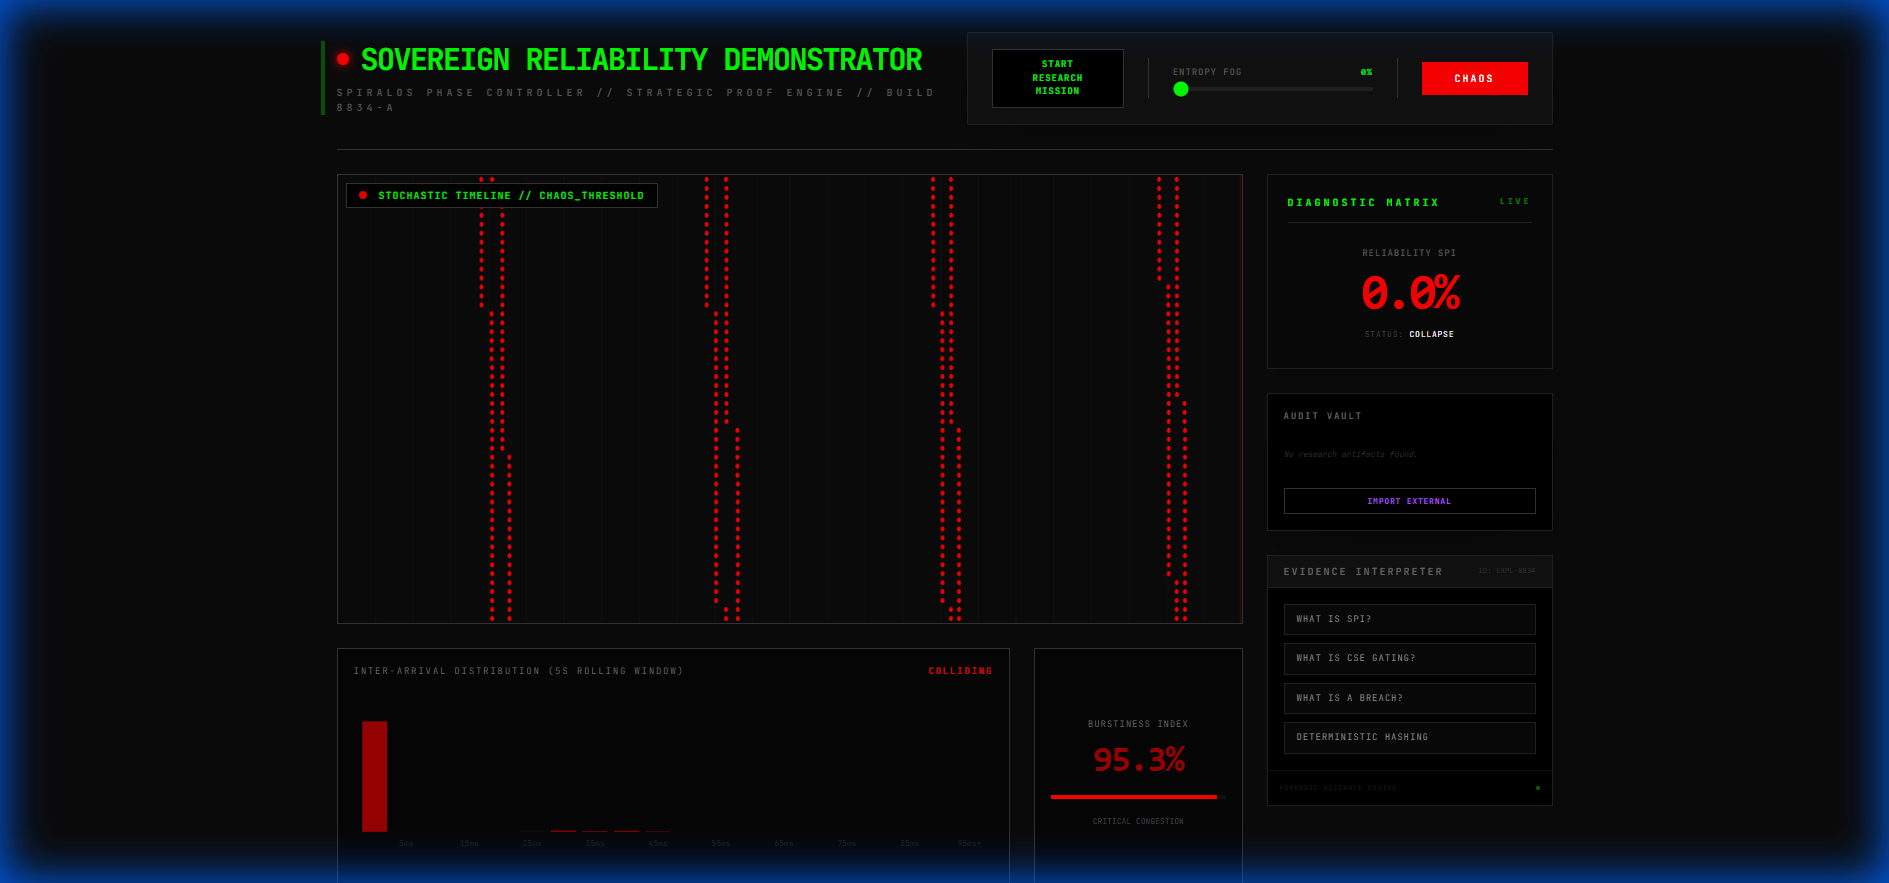
\includegraphics[width=\linewidth]{chaos_mode.png}
\caption{Control state (no phase control): synchronized execution produces a high-density burst wall.}
\label{fig:chaos}
\end{figure}

\subsection{Phase-Controlled State (Order / Dispersion)}
With Phase Controller active, executions distribute across the scheduling window. The inter-arrival histogram trends toward a bounded uniform dispersion.

\begin{figure}[t]
\centering
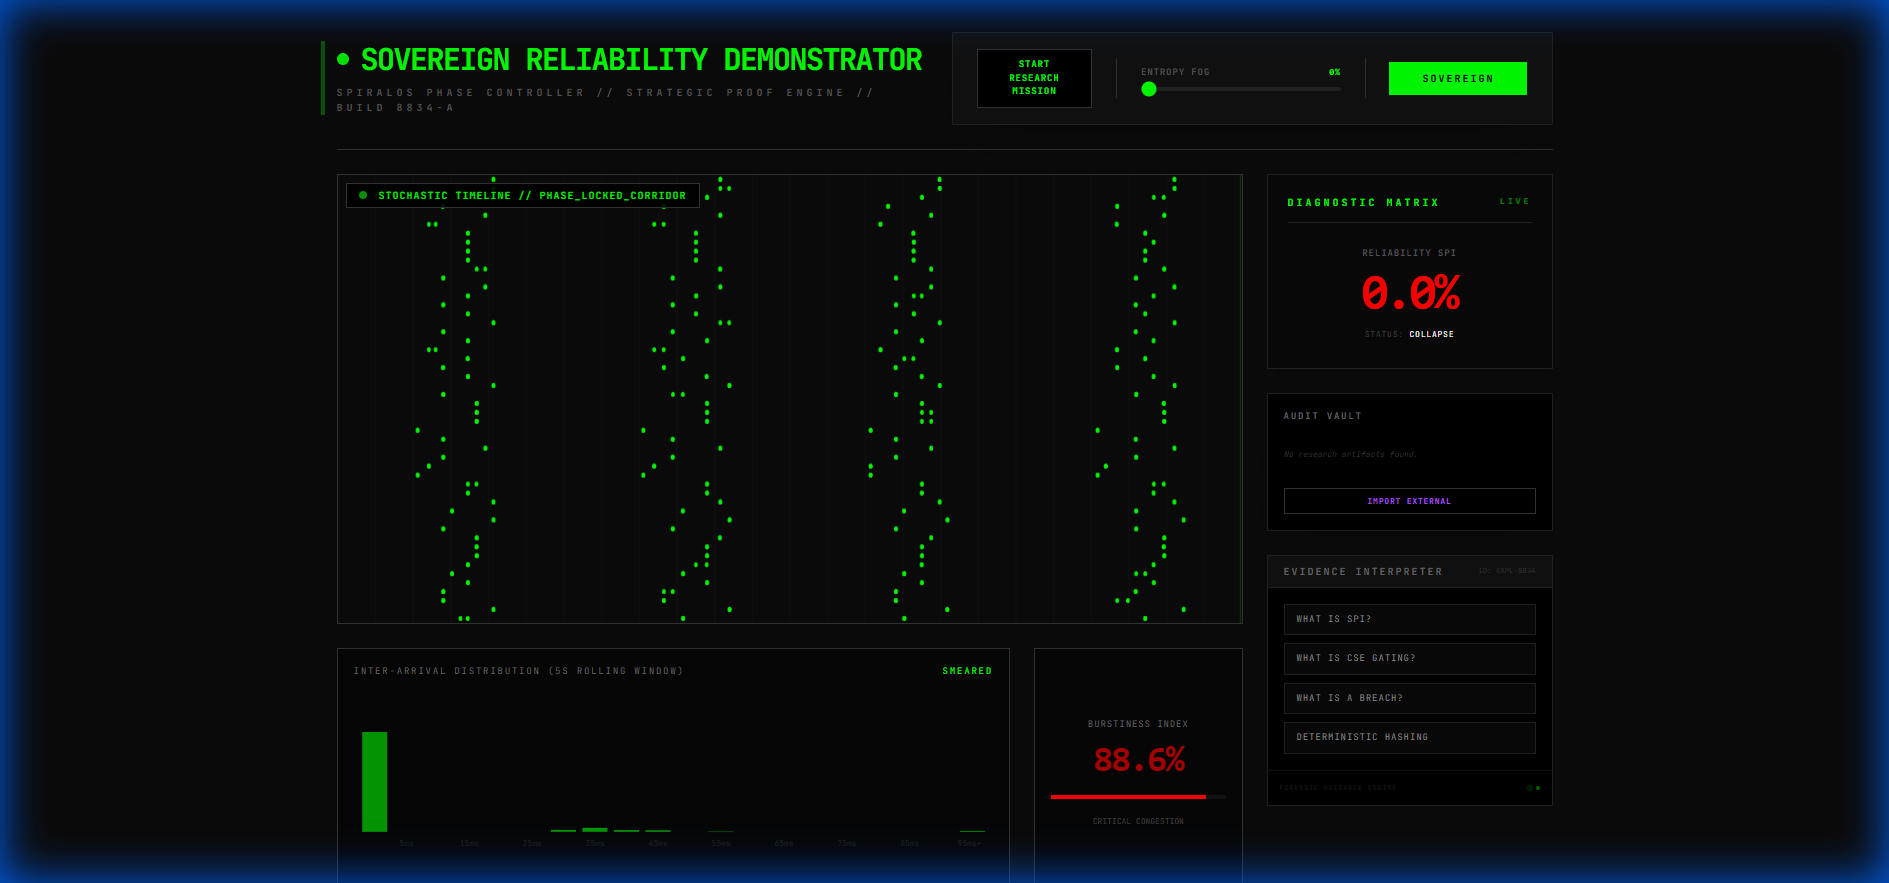
\includegraphics[width=\linewidth]{order_mode.png}
\caption{Phase-controlled state: distributed execution wavefront (``Green Highway'') under variance injection.}
\label{fig:order}
\end{figure}

% =========================================================
\section{Results and Discussion}

\subsection{The ``Green Highway'' Corridor}
A key observed behavior is corridor preservation: under injected variance, the execution pattern broadens into a structured band rather than collapsing into a burst cluster. This indicates that a deterministic scheduling skeleton can constrain noise into an interpretable corridor.

\subsection{Auditability and Evidence Gating}
The demonstrator includes a cold audit pipeline that re-derives metrics and applies certification gates. If determinism is compromised or evidence density is insufficient (e.g., headless runs, excessive entropy), the system returns an explicit non-certifying state rather than issuing a false pass.

\noindent \textbf{Design rule:} \emph{Refusal to certify is a valid outcome.}

% =========================================================
\section{Implications for Defense and Regulated Systems}
Deterministic fleet dispersion under variance has direct implications for:

\begin{itemize}
\item \textbf{Predictable C2 Slots:} scheduling control-plane traffic to reduce collisions.
\item \textbf{Forensic Replay:} separating logic defects from transport anomalies.
\item \textbf{Assurance Posture:} reducing PRNG reliance in critical scheduling paths.
\end{itemize}

% =========================================================
\section{Conclusion}
Deterministic phase control provides a low-complexity mechanism to mitigate herd behavior without injecting stochastic uncertainty into high-assurance workflows. By replacing randomized backoff with hash-derived scheduling offsets, the system converts synchronized recovery from an uncontrolled threat into a bounded resource.

\section*{Availability}
\noindent Source repository: \url{https://github.com/ZoaGrad/sovereign-reliability-lab}\\
Maintained by Blackglass Continuum LLC (CAGE: 17TJ5).\\
UNCLASSIFIED // PUBLIC RELEASE.

% =========================================================
\section*{References}
\begin{enumerate}
\item Beyer, B., Jones, C., Petoff, J., \& Murphy, N. (2016). \textit{Site Reliability Engineering: How Google Runs Production Systems}. O'Reilly Media.
\item NIST. (2020). \textit{Zero Trust Architecture (SP 800-207)}. National Institute of Standards and Technology.
\item Willis, C. (2026). \textit{Sovereign Reliability Lab: Evidence Bundles and Audit Artifacts}. Blackglass Continuum LLC.
\end{enumerate}

\end{document}
